\section{Automatic generation of JIT compilers}

Traditional JIT compilers are hard to write, time consuming, hard to evolve,
etc. etc.

\begin{figure}[h]
\begin{center}
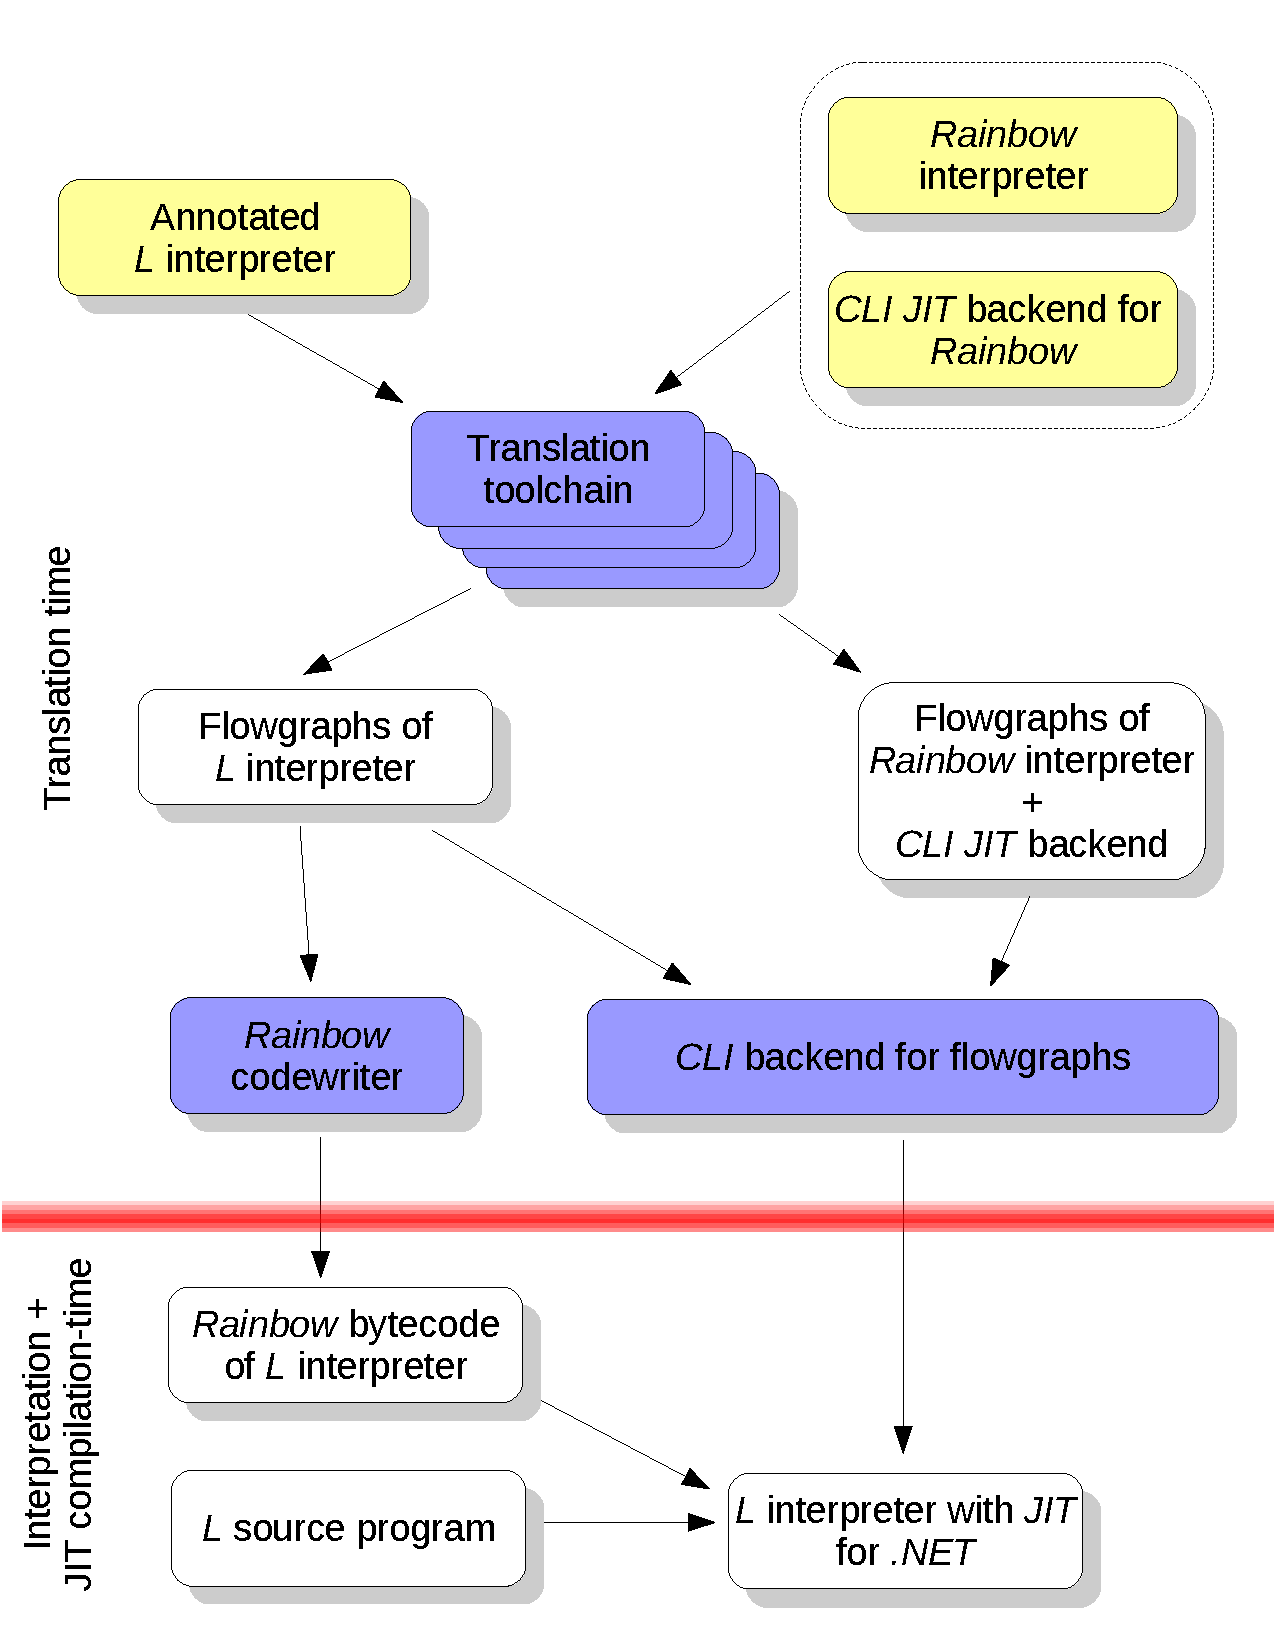
\includegraphics[width=.6\textwidth]{diagram1}
\caption{PyPy infrastructure for generating an interpreter of a
  language $L$ with JIT compilation for the .NET platform}
\end{center}
\end{figure}

The JIT generation framework uses partial evaluation techniques to generate a
dynamic compiler from an interpreter; the idea is inspired by Psyco, which
uses the same techniques but it's manually written instead of being
automatically generated.

The original idea is by Futamura \cite{Futamura99}. He proposed to generate compilers
from interpreters with automatic specialization, but his work has had
relatively little practical impact so far.

\subsection{Partial evaluation}

Assume the Python bytecode to be constant, and constant-propagate it into the
Python interpreter.

Example::
\begin{lstlisting}[language=Python]
  def f(x, y):    
    x2 = x * x    
    y2 = y * y    
    return x2 + y2

**case x=3** ::

  def f_3(y):    
    y2 = y * y   
    return 9 + y2

**case x=10** ::

  def f_10(y):    
    y2 = y * y   
    return 100 + y2
\end{lstlisting}

A shortcoming of PE is that in many cases not much can be really assumed
constant at compile-time, and this leads to poor results.  Effective dynamic
compilation requires feedback of runtime information into compile-time; for a
dynamic language, types are a primary example.


\subsection{Execution steps}

* Translation time

  - pypy-c-jit is translated into an executable

  - the JIT compiler is automatically generated

* Compile-time: the JIT compiler runs

* Runtime: the JIT compiled code runs

* Compile-time and runtime are intermixed
